\documentclass[12pt, a4paper]{article}
\usepackage[utf8]{inputenc}
\usepackage[T1]{fontenc}
\usepackage[french]{babel}
\usepackage{graphicx}
\usepackage{fancyhdr}
\usepackage{geometry}
\usepackage{listings}
\usepackage{xcolor}
\usepackage{float}
\usepackage{tcolorbox}
\usepackage{enumitem}

\usepackage[
    bookmarks=true,
    bookmarksopen=true,
    bookmarksnumbered=true,
    pdfusetitle,
    colorlinks=true,
    linkcolor=blue,
    urlcolor=blue,
    pdfborder={0 0 0}
]{hyperref}

\geometry{top=2.5cm, bottom=2.5cm, left=2.5cm, right=2.5cm}

% Configuration des listes
\setlist[itemize]{itemsep=0.5em, parsep=0.3em}
\setlist[enumerate]{itemsep=0.5em, parsep=0.3em}

% Définition des couleurs pour le code
\definecolor{codegreen}{rgb}{0,0.6,0}
\definecolor{codegray}{rgb}{0.5,0.5,0.5}
\definecolor{codepurple}{rgb}{0.58,0,0.12}
\definecolor{backcolour}{rgb}{0.95,0.95,0.92}

% Configuration du style de code
\lstdefinestyle{formulastyle}{
    backgroundcolor=\color{backcolour},   
    commentstyle=\color{codegreen},
    keywordstyle=\color{magenta},
    numberstyle=\tiny\color{codegray},
    stringstyle=\color{codepurple},
    basicstyle=\ttfamily\footnotesize,
    breakatwhitespace=false,         
    breaklines=true,                 
    captionpos=b,                    
    keepspaces=true,                 
    showspaces=false,                
    showstringspaces=false,
    showtabs=false,                  
    tabsize=2,
    frame=single,
    literate={é}{{\'e}}1 {è}{{\`e}}1 {à}{{\`a}}1 {ç}{{\c{c}}}1 {ù}{{\`u}}1 {ê}{{\^e}}1 {î}{{\^i}}1 {ô}{{\^o}}1 {û}{{\^u}}1 {ë}{{\¨e}}1 {ï}{{\¨i}}1 {ü}{{\¨u}}1 {Ç}{{\c{C}}}1
}

\lstset{style=formulastyle}

% Définition des styles de boîtes
\newtcolorbox{note}{
    colback=blue!5,
    colframe=blue!75!black,
    title=Note,
    fonttitle=\bfseries
}

\newtcolorbox{warning}{
    colback=red!5,
    colframe=red!75!black,
    title=Attention !,
    fonttitle=\bfseries
}

\newtcolorbox{tip}{
    colback=green!5,
    colframe=green!75!black,
    title=Astuce,
    fonttitle=\bfseries
}

\makeatletter
\def\maketitle{
    \begin{titlepage}
        \centering
        \vspace*{2cm}
        
        % Logo
        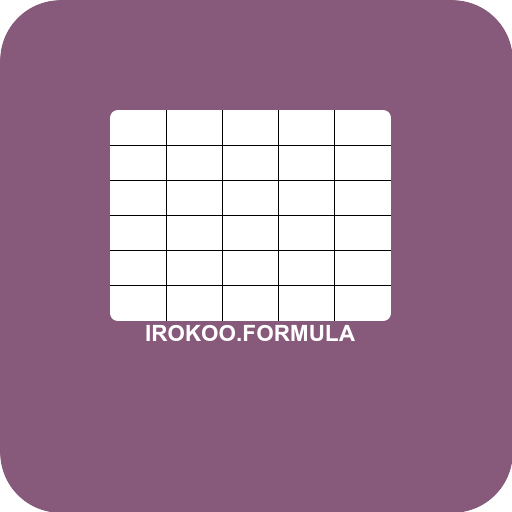
\includegraphics[width=0.4\textwidth]{../icon.png}
        \vspace{2cm}
        
        % Titre
        {\huge\bfseries Documentation Formules\\Spreadsheet Evolution\par}
        \vspace{2cm}
        
        % Auteur
        {\Large\itshape Sylvain Boutet\par}
        \vspace{1cm}
        
        % Date
        {\large \@date\par}
        
        \vfill
        
        % Pied de page
        {\large Odoo Version 18.0\par}
    \end{titlepage}
}
\makeatother

\title{Documentation des Formules Odoo Spreadsheet}
\author{IROKOO}
\date{\today}

% Début du document
\begin{document}

\maketitle
\tableofcontents
\newpage

\section{Introduction}

Le module \textbf{Spreadsheet Evolution} étend les fonctionnalités des feuilles de calcul Odoo en ajoutant des formules avancées permettant d'exploiter pleinement les données du système directement dans vos spreadsheets sans export préalable.

Ces formules permettent :
\begin{itemize}
    \item L'accès direct aux champs de n'importe quel enregistrement dans Odoo
    \item La recherche conditionnelle d'enregistrements avec des filtres avancés
    \item L'agrégation de données (sommes, moyennes, etc.)
    \item Les regroupements sophistiqués
    \item Le calcul direct de sommes avec des domaines de filtrage
\end{itemize}

\begin{figure}[H]
    \centering
    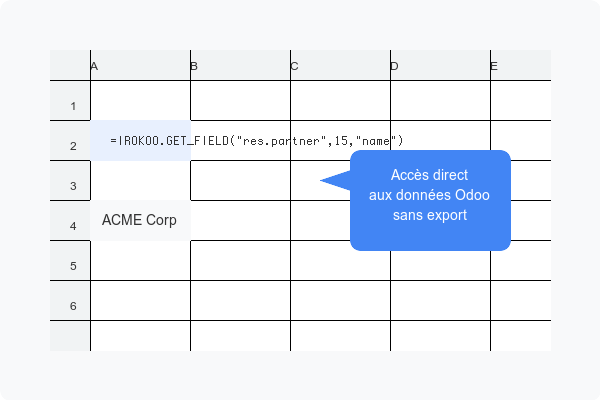
\includegraphics[width=0.6\textwidth]{feature1.png}
    \caption{Exemple d'utilisation des formules dans une feuille de calcul}
\end{figure}

\section{Liste des formules disponibles}

\subsection{IROKOO.GET\_FIELD}
\begin{tcolorbox}[title=Description]
Récupère la valeur d'un champ spécifique pour un enregistrement donné dans n'importe quel modèle Odoo.
\end{tcolorbox}

\subsubsection{Syntaxe}
\begin{lstlisting}
=IROKOO.GET_FIELD(model, id, field)
\end{lstlisting}

\subsubsection{Paramètres}
\begin{itemize}
    \item \textbf{model} (chaîne) : Nom technique du modèle (ex: "res.partner")
    \item \textbf{id} (nombre) : ID de l'enregistrement
    \item \textbf{field} (chaîne) : Nom technique du champ (ex: "name", "email", "phone")
\end{itemize}

\subsubsection{Retourne}
La valeur du champ demandé.

\subsubsection{Exemple}
\begin{lstlisting}
=IROKOO.GET_FIELD("res.partner", 1, "name")
\end{lstlisting}
Retourne le nom du partenaire ayant l'ID 1.

\subsubsection{Exemple avec champ relationnel}
\begin{lstlisting}
=IROKOO.GET_FIELD("sale.order", 123, "partner_id.name")
\end{lstlisting}
Retourne directement le nom du client associé à la commande de vente ayant l'ID 123, en accédant au champ \texttt{name} à travers la relation \texttt{partner\_id}.

\begin{tip}
Cette formule fonctionne avec tous les types de champs, y compris les champs relationnels. Pour les champs relationnels, le contenu retourné sera automatiquement formaté de manière appropriée.
\end{tip}

\subsection{IROKOO.GET\_IDS}
\begin{tcolorbox}[title=Description]
Récupère les IDs des enregistrements d'un modèle qui correspondent aux critères de filtre spécifiés.
\end{tcolorbox}

\subsubsection{Syntaxe}
\begin{lstlisting}
=IROKOO.GET_IDS(model, order, direction, limit, filters)
\end{lstlisting}

\subsubsection{Paramètres}
\begin{itemize}
    \item \textbf{model} (chaîne) : Nom technique du modèle (ex: "sale.order")
    \item \textbf{order} (chaîne) : Champ pour le tri (ex: "date\_order")
    \item \textbf{direction} (chaîne) : Direction du tri ("asc" ou "desc")
    \item \textbf{limit} (nombre) : Nombre maximum d'enregistrements à retourner (0 pour pas de limite)
    \item \textbf{filters} (chaîne) : Filtres séparés par des points-virgules
\end{itemize}

\subsubsection{Formats de filtre supportés}
\begin{itemize}
    \item \textbf{Format explicite} : \texttt{field:operator:value}
    \begin{itemize}
        \item Exemple : \texttt{state:in:draft,sent}
        \item Opérateurs : \texttt{=}, \texttt{!=}, \texttt{>}, \texttt{<}, \texttt{>=}, \texttt{<=}, \texttt{in}, \texttt{not in}, \texttt{ilike}, \texttt{like}
    \end{itemize}
    \item \textbf{Format simple} : \texttt{field=value}, \texttt{field>value}, etc.
    \begin{itemize}
        \item Exemple : \texttt{amount\_total>1000}
    \end{itemize}
    \item \textbf{Format recherche texte} : \texttt{field~value} pour recherches insensibles à la casse
    \begin{itemize}
        \item Exemple : \texttt{name~Comptabilité}
    \end{itemize}
    \item \textbf{Format avec \%} : \texttt{field=\%valeur\%} pour recherches partielles
    \begin{itemize}
        \item Exemple : \texttt{name=\%Dupont\%}
    \end{itemize}
\end{itemize}

\subsubsection{Retourne}
Une chaîne contenant les IDs séparés par des virgules.

\subsubsection{Exemple}
\begin{lstlisting}
=IROKOO.GET_IDS("sale.order", "date_order", "desc", 10, "state:in:draft,sent;date_order>2023-01-01")
\end{lstlisting}
Retourne les 10 derniers devis/commandes en état brouillon ou envoyé créés après le 1er janvier 2023.

\begin{warning}
Pour les filtres contenant des caractères spéciaux, assurez-vous d'utiliser le format explicite avec des deux-points comme séparateurs.
\end{warning}

\subsection{IROKOO.GET\_SUM}
\begin{tcolorbox}[title=Description]
Calcule la somme des valeurs d'un champ pour une liste d'IDs.
\end{tcolorbox}

\subsubsection{Syntaxe}
\begin{lstlisting}
=IROKOO.GET_SUM(model, field, ids)
\end{lstlisting}

\subsubsection{Paramètres}
\begin{itemize}
    \item \textbf{model} (chaîne) : Nom technique du modèle (ex: "sale.order")
    \item \textbf{field} (chaîne) : Nom technique du champ à sommer (ex: "amount\_untaxed")
    \item \textbf{ids} (chaîne) : Liste d'IDs séparés par des virgules (généralement le résultat de GET\_IDS)
\end{itemize}

\subsubsection{Retourne}
La somme des valeurs du champ pour les enregistrements spécifiés.

\subsubsection{Exemple}
\begin{lstlisting}
=IROKOO.GET_SUM("sale.order", "amount_untaxed", IROKOO.GET_IDS("sale.order", "date_order", "desc", 0, "state=sale"))
\end{lstlisting}
Calcule la somme des montants HT de toutes les commandes confirmées.

\begin{note}
Cette formule est particulièrement utile combinée avec GET\_IDS pour créer des rapports dynamiques.
\end{note}

\subsection{IROKOO.GET\_GROUPED\_IDS}
\begin{tcolorbox}[title=Description]
Regroupe les enregistrements selon un champ et calcule une valeur agrégée pour chaque groupe.
\end{tcolorbox}

\subsubsection{Syntaxe}
\begin{lstlisting}
=IROKOO.GET_GROUPED_IDS(model, group_by, aggregate_field, aggregate_function, filters, limit)
\end{lstlisting}

\subsubsection{Paramètres}
\begin{itemize}
    \item \textbf{model} (chaîne) : Nom technique du modèle
    \item \textbf{group\_by} (chaîne) : Champ utilisé pour le regroupement
    \item \textbf{aggregate\_field} (chaîne) : Champ à agréger
    \item \textbf{aggregate\_function} (chaîne) : Fonction d'agrégation : "sum", "avg", "count", "min", "max"
    \item \textbf{filters} (chaîne) : Filtres (même format que GET\_IDS)
    \item \textbf{limit} (nombre) : Nombre maximum de groupes à retourner
\end{itemize}

\subsubsection{Retourne}
Une chaîne contenant les valeurs du champ de regroupement, séparées par des virgules, pour les groupes classés par valeur agrégée décroissante.

\subsubsection{Exemple}
\begin{lstlisting}
=IROKOO.GET_GROUPED_IDS("sale.order", "partner_id", "amount_total", "sum", "state=sale", 5)
\end{lstlisting}
Retourne les IDs des 5 clients ayant généré le plus de chiffre d'affaires à travers les commandes confirmées.

\begin{tip}
Cette formule est idéale pour créer des analyses de type "Top N" ou pour identifier des tendances comme les clients les plus actifs, les produits les plus vendus, etc.
\end{tip}

\subsection{IROKOO.SUM\_BY\_DOMAIN}
\begin{tcolorbox}[title=Description]
Calcule directement la somme d'un champ pour les enregistrements correspondant à un domaine, sans nécessiter d'étape intermédiaire.
\end{tcolorbox}

\subsubsection{Syntaxe}
\begin{lstlisting}
=IROKOO.SUM_BY_DOMAIN(model, field, filters)
\end{lstlisting}

\subsubsection{Paramètres}
\begin{itemize}
    \item \textbf{model} (chaîne) : Nom technique du modèle
    \item \textbf{field} (chaîne) : Champ à sommer
    \item \textbf{filters} (chaîne) : Filtres (même format que GET\_IDS)
\end{itemize}

\subsubsection{Retourne}
La somme des valeurs du champ pour les enregistrements correspondant aux filtres.

\subsubsection{Exemple}
\begin{lstlisting}
=IROKOO.SUM_BY_DOMAIN("account.move.line", "balance", "account_id=401100;date>=2023-01-01;date<=2023-12-31")
\end{lstlisting}
Calcule le solde total des écritures comptables sur le compte fournisseurs 401100 pour l'année 2023.

\begin{figure}[H]
    \centering
    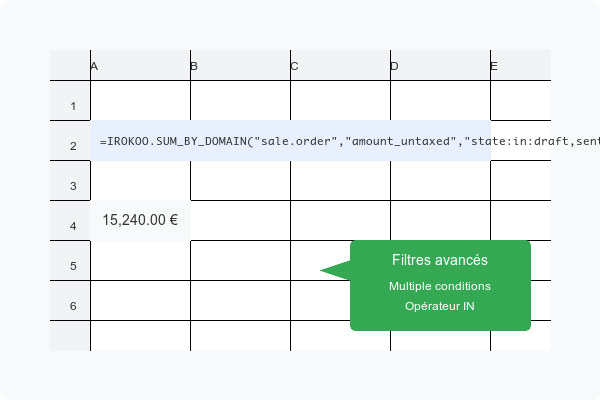
\includegraphics[width=0.8\textwidth]{feature2.png}
    \caption{Exemple d'utilisation de SUM\_BY\_DOMAIN avec filtres complexes}
\end{figure}

\section{Utilisation avancée}

\subsection{Combinaison de formules}
Les formules peuvent être combinées pour créer des analyses complexes :
\begin{lstlisting}
=IROKOO.GET_SUM("sale.order", "amount_untaxed", 
  IROKOO.GET_IDS("sale.order", "date_order", "desc", 0, 
    "state=sale;partner_id=" & IROKOO.GET_GROUPED_IDS("sale.order", "partner_id", "amount_total", "sum", "state=sale", 1)
  )
)
\end{lstlisting}
Cette formule calcule le montant total des ventes pour le meilleur client.

\subsection{Filtres avec l'opérateur IN}
Utilisez l'opérateur IN pour filtrer sur plusieurs valeurs :
\begin{lstlisting}
=IROKOO.SUM_BY_DOMAIN("sale.order", "amount_total", "state:in:draft,sent,sale;date>=2023-01-01")
\end{lstlisting}

\subsection{Conseils pour les performances}
\begin{itemize}
    \item Limiter le nombre d'appels de formules en utilisant SUM\_BY\_DOMAIN directement quand possible
    \item Utiliser des limites appropriées dans GET\_IDS pour réduire le volume de données
    \item Réutiliser les résultats de GET\_IDS dans plusieurs cellules plutôt que de répéter l'appel
    \item Préférer le format explicite field:operator:value pour les filtres complexes
\end{itemize}

\subsection{Utilisation de cellules de référence comme filtres}

Il est important de noter que les formules IROKOO.* ne sont pas directement compatibles avec les filtres globaux natifs d'Odoo Spreadsheet. Cependant, vous pouvez créer un système de filtrage efficace en utilisant des cellules de référence :

\begin{itemize}
    \item \textbf{Pour l'année} : Créez une cellule avec validation de données (liste déroulante) contenant les années disponibles, et référencez cette cellule dans vos formules
    \item \textbf{Pour la période} : Utilisez des cellules pour définir les dates de début et de fin, qui serviront de paramètres à toutes vos formules
    \item \textbf{Pour d'autres filtres} : Créez des cellules contenant les IDs des équipes, produits, etc., que vous souhaitez filtrer
\end{itemize}

Exemple de mise en place :
\begin{lstlisting}
D1: "Filtre par équipe"
D2: [liste déroulante avec IDs des équipes]
\end{lstlisting}

Puis dans vos formules, référencez cette cellule :
\begin{lstlisting}
=IROKOO.SUM_BY_DOMAIN("sale.order", "amount_untaxed", "state=sale;team_id=" & D2 & ";date_order>=" & TEXT(B2,"yyyy-mm-dd"))
\end{lstlisting}

Cette approche permet de mettre à jour dynamiquement toutes vos formules lorsque l'utilisateur change la valeur d'une cellule de filtrage.

\subsection{Conseils pour l'optimisation}

\begin{itemize}
    \item Utilisez des cellules de référence pour les paramètres communs (dates, filtres)
    \item Minimisez le nombre d'appels à IROKOO.GET\_IDS en stockant les résultats dans des cellules intermédiaires
    \item Privilégiez IROKOO.SUM\_BY\_DOMAIN pour les calculs directs plutôt que des formules imbriquées complexes
    \item Pour les tableaux très volumineux, segmentez vos requêtes par période pour améliorer les performances
\end{itemize}

Ce tableau de bord vous donne un point de départ pour créer vos propres analyses adaptées à vos besoins spécifiques. Les formules peuvent être modifiées et combinées pour répondre à différentes questions métier.

\section{Dépannage}

\subsection{Erreurs courantes}
\begin{itemize}
    \item \textbf{"All parameters are required"} : Vérifiez que tous les arguments obligatoires sont fournis
    \item \textbf{"Loading data..."} : Patientez, les données sont en cours de chargement
    \item \textbf{"No results found"} : Les filtres ne correspondent à aucun enregistrement
    \item \textbf{"Error while executing search"} : Vérifiez la syntaxe des filtres et l'existence du modèle
\end{itemize}

\subsection{Problèmes d'accès}
\begin{itemize}
    \item Les formules respectent les droits d'accès de l'utilisateur
    \item Un utilisateur ne peut accéder qu'aux données auxquelles il a droit
    \item Si une formule retourne une erreur pour certains utilisateurs, vérifiez leurs droits d'accès
\end{itemize}

\begin{warning}
Si vous rencontrez des problèmes d'accès, assurez-vous que l'utilisateur a les droits nécessaires pour accéder au modèle et aux champs spécifiés dans la formule.
\end{warning}

\section{Exemple de tableau de bord}

Cette section présente un exemple complet de construction d'un tableau de bord d'analyse des ventes à l'aide des formules du module Spreadsheet Evolution.

\subsection{Objectif du tableau de bord}

Notre tableau de bord vise à répondre aux questions suivantes :
\begin{itemize}
    \item Quelle est l'évolution mensuelle des ventes sur l'année en cours ?
    \item Qui sont nos 5 meilleurs clients et leur chiffre d'affaires ?
    \item Quels sont nos 5 produits les plus vendus (en valeur et en quantité) ?
    \item Quel est le taux de conversion de nos devis en commandes ?
    \item Comment se répartissent nos ventes par équipe de vente ?
\end{itemize}


\subsection{Implémentation étape par étape}

\subsubsection{Étape 1 : Préparation des données de référence}

Commençons par créer des cellules de référence pour les dates et filtres :

\begin{lstlisting}
A1: "Année en cours"
B1: =YEAR(TODAY())
A2: "Date début"
B2: =DATE(B1,1,1)
A3: "Date fin"
B3: =DATE(B1,12,31)
\end{lstlisting}

\subsubsection{Étape 2 : Évolution mensuelle des ventes}

Pour créer l'évolution mensuelle, nous allons calculer le total pour chaque mois :

\begin{lstlisting}
A5: "Mois"
B5: "Total ventes HT"
C5: "Nombre de commandes"

A6: "Janvier"
B6: =IROKOO.SUM_BY_DOMAIN("sale.order", "amount_untaxed", "state=sale;date_order>=" & TEXT(DATE(B1,1,1),"yyyy-mm-dd") & ";date_order<=" & TEXT(DATE(B1,1,31),"yyyy-mm-dd"))
C6: =IROKOO.SUM_BY_DOMAIN("sale.order", "1", "state=sale;date_order>=" & TEXT(DATE(B1,1,1),"yyyy-mm-dd") & ";date_order<=" & TEXT(DATE(B1,1,31),"yyyy-mm-dd"))

A7: "Février"
B7: =IROKOO.SUM_BY_DOMAIN("sale.order", "amount_untaxed", "state=sale;date_order>=" & TEXT(DATE(B1,2,1),"yyyy-mm-dd") & ";date_order<=" & TEXT(DATE(B1,2,28),"yyyy-mm-dd"))
C7: =IROKOO.SUM_BY_DOMAIN("sale.order", "1", "state=sale;date_order>=" & TEXT(DATE(B1,2,1),"yyyy-mm-dd") & ";date_order<=" & TEXT(DATE(B1,2,28),"yyyy-mm-dd"))

# Répéter pour tous les mois...
\end{lstlisting}

\subsubsection{Étape 3 : Top 5 clients}

Identifions nos meilleurs clients par chiffre d'affaires :

\begin{lstlisting}
E5: "Top 5 clients"
F5: "CA Total HT"

# Obtenir les IDs des 5 meilleurs clients
E6: =IROKOO.GET_FIELD("res.partner", SPLIT(IROKOO.GET_GROUPED_IDS("sale.order", "partner_id", "amount_total", "sum", "state=sale;date_order>=" & TEXT(B2,"yyyy-mm-dd") & ";date_order<=" & TEXT(B3,"yyyy-mm-dd"), 1), ","), "name")
F6: =IROKOO.SUM_BY_DOMAIN("sale.order", "amount_untaxed", "state=sale;partner_id=" & SPLIT(IROKOO.GET_GROUPED_IDS("sale.order", "partner_id", "amount_total", "sum", "state=sale;date_order>=" & TEXT(B2,"yyyy-mm-dd") & ";date_order<=" & TEXT(B3,"yyyy-mm-dd"), 1), ",") & ";date_order>=" & TEXT(B2,"yyyy-mm-dd") & ";date_order<=" & TEXT(B3,"yyyy-mm-dd"))

# Répéter pour les 4 autres clients (rangs 2 à 5)...
\end{lstlisting}

\subsubsection{Étape 4 : Top 5 produits}

Analysons les produits les plus performants :

\begin{lstlisting}
H5: "Top 5 produits"
I5: "Quantité vendue"
J5: "CA Total HT"

# Obtenir les données du premier produit
H6: =IROKOO.GET_FIELD("product.product", SPLIT(IROKOO.GET_GROUPED_IDS("sale.order.line", "product_id", "price_subtotal", "sum", "order_id.state=sale;order_id.date_order>=" & TEXT(B2,"yyyy-mm-dd") & ";order_id.date_order<=" & TEXT(B3,"yyyy-mm-dd"), 1), ","), "name")
I6: =IROKOO.SUM_BY_DOMAIN("sale.order.line", "product_uom_qty", "order_id.state=sale;product_id=" & SPLIT(IROKOO.GET_GROUPED_IDS("sale.order.line", "product_id", "price_subtotal", "sum", "order_id.state=sale;order_id.date_order>=" & TEXT(B2,"yyyy-mm-dd") & ";order_id.date_order<=" & TEXT(B3,"yyyy-mm-dd"), 1), ",") & ";order_id.date_order>=" & TEXT(B2,"yyyy-mm-dd") & ";order_id.date_order<=" & TEXT(B3,"yyyy-mm-dd"))
J6: =IROKOO.SUM_BY_DOMAIN("sale.order.line", "price_subtotal", "order_id.state=sale;product_id=" & SPLIT(IROKOO.GET_GROUPED_IDS("sale.order.line", "product_id", "price_subtotal", "sum", "order_id.state=sale;order_id.date_order>=" & TEXT(B2,"yyyy-mm-dd") & ";order_id.date_order<=" & TEXT(B3,"yyyy-mm-dd"), 1), ",") & ";order_id.date_order>=" & TEXT(B2,"yyyy-mm-dd") & ";order_id.date_order<=" & TEXT(B3,"yyyy-mm-dd"))

# Répéter pour les 4 autres produits...
\end{lstlisting}

\subsubsection{Étape 5 : Taux de conversion des devis}

Calculons le taux de conversion des devis en commandes :

\begin{lstlisting}
A18: "Taux de conversion des devis"
A19: "Nombre total de devis"
B19: =IROKOO.SUM_BY_DOMAIN("sale.order", "1", "date_order>=" & TEXT(B2,"yyyy-mm-dd") & ";date_order<=" & TEXT(B3,"yyyy-mm-dd"))
A20: "Nombre de commandes confirmées"
B20: =IROKOO.SUM_BY_DOMAIN("sale.order", "1", "state=sale;date_order>=" & TEXT(B2,"yyyy-mm-dd") & ";date_order<=" & TEXT(B3,"yyyy-mm-dd"))
A21: "Taux de conversion"
B21: =B20/B19
\end{lstlisting}

\subsubsection{Étape 6 : Répartition par équipe de vente}

Analysons les performances par équipe de vente :

\begin{lstlisting}
E18: "Répartition par équipe de vente"
F18: "CA Total HT"
G18: "Nombre de commandes"

# Obtenir les équipes de vente
E19: =IROKOO.GET_FIELD("crm.team", SPLIT(IROKOO.GET_GROUPED_IDS("sale.order", "team_id", "amount_total", "sum", "state=sale;date_order>=" & TEXT(B2,"yyyy-mm-dd") & ";date_order<=" & TEXT(B3,"yyyy-mm-dd"), 1), ","), "name")
F19: =IROKOO.SUM_BY_DOMAIN("sale.order", "amount_untaxed", "state=sale;team_id=" & SPLIT(IROKOO.GET_GROUPED_IDS("sale.order", "team_id", "amount_total", "sum", "state=sale;date_order>=" & TEXT(B2,"yyyy-mm-dd") & ";date_order<=" & TEXT(B3,"yyyy-mm-dd"), 1), ",") & ";date_order>=" & TEXT(B2,"yyyy-mm-dd") & ";date_order<=" & TEXT(B3,"yyyy-mm-dd"))
G19: =IROKOO.SUM_BY_DOMAIN("sale.order", "1", "state=sale;team_id=" & SPLIT(IROKOO.GET_GROUPED_IDS("sale.order", "team_id", "amount_total", "sum", "state=sale;date_order>=" & TEXT(B2,"yyyy-mm-dd") & ";date_order<=" & TEXT(B3,"yyyy-mm-dd"), 1), ",") & ";date_order>=" & TEXT(B2,"yyyy-mm-dd") & ";date_order<=" & TEXT(B3,"yyyy-mm-dd"))

# Répéter pour les autres équipes...
\end{lstlisting}

\subsection{Ajout de graphiques}

Pour rendre le tableau de bord plus visuel, ajoutez des graphiques :

\begin{itemize}
    \item Un graphique en colonnes pour l'évolution mensuelle des ventes
    \item Un graphique en secteurs pour la répartition des ventes par équipe
    \item Un graphique en barres horizontales pour les top 5 clients et produits
\end{itemize}

Ce tableau de bord vous donne un point de départ pour créer vos propres analyses adaptées à vos besoins spécifiques. Les formules peuvent être modifiées et combinées pour répondre à différentes questions métier.

\end{document} 